\documentclass[12pt, letterpaper]{article}
\usepackage[utf8]{inputenc}
\usepackage{mathtools}
\usepackage{indentfirst}
\usepackage{hyperref}
\usepackage{pgfplots}
\usepackage{listings}
\pgfplotsset{compat=1.9, width=10cm}

\usepgfplotslibrary{external}
\tikzexternalize

\DeclarePairedDelimiter\abs{\lvert}{\rvert}%

\title{Trabalho Prático 3}
\author{Hugo Silva, José Torres}
\date{novembro 2022}

\begin{document}

\maketitle

\section*{Introdução}

Visamos estudar métodos de aproximação numéricos para o cálculo de valores exatos de $f(x)$, sendo $f$ a função em questão.

Durante este trabalho iremos usufruir de \textbf{métodos de interpolação} de funções e usufruiremos também de \textbf{métodos de construção de splines} (maioritariamente cúbicas) para tais funções. 

\section*{Exercício 1}

A função a ser estudade é $f(x) = x^2 + \sin(6x)$ para $x \in \mathopen[-1,1\mathclose]$

\begin{quote}
\centering
    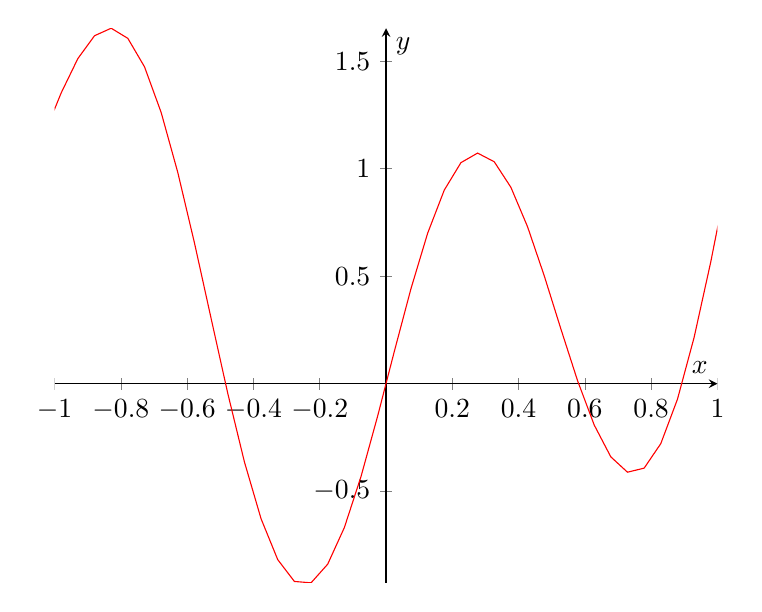
\begin{tikzpicture}
        \begin{axis} [xmin=-1, xmax=1, axis lines=middle, xlabel=$x$, ylabel=$y$]
            \addplot[color=red, samples=200]{x^2 + sin(deg(6*x))};
        \end{axis}
    \end{tikzpicture}
\end{quote}

\begin{itemize}
    \item Pretende-se calcular um conjunto $n+1 = 8$ pontos, ($x_i, f_i = f(x_i)$) inicialmente. \\
    
    Para tal, calculamos atribui-se $x_0 = -1$ e $x_7 = 1$ e, consequentemente, todos os pontos intermédios irão estar divididos em parcelas aproximadamente iguais entre $x_0 e x_7$, parcelas essas que podem ser calculadas através da amplitude $h$:

    \[h = \frac{b-a}{n}\]

    Onde $\mathopen[-1,1\mathclose] = \mathopen[a,b\mathclose]$ e $n = 7$. \\
    
    Da fórmula acima indicada temos o desenvolvimento:

    \[h = \frac{1-(-1)}{7} = \frac{2}{7} \approx 0.286\]

    E finalmente temos que:

    \[x_n = x_0 + h\times n \Leftrightarrow x_n = -1 + 0.286n\]

    Por fim obtemos a tabela de valores:
    
    \begin{center}
        \begin{tabular} {|| c | c | c | c | c | c | c | c | c ||} \hline
            $i$ & $0$ & $1$ & $2$ & $3$ & $4$ & $5$ & $6$ & $7$\\ [0.4ex]\hline
            $x_i$ & $-1$ & $-0.714$ & $-0.428$ & $-0.142$ & $0.144$ & $0.430$ & $0.716$ & $1$ \\ [0.4ex]\hline
        \end{tabular}
    \end{center}

    \textbf{\textit{NOTA:}} Os valores de $x_i$ são arredondados devido ao facto da amplitude resultar de um valor aproximado, portanto o intervalo entre $[0.716,1]$ é mais pequeno do que o intervalo entre $[0.430, 0.716]$, porém não é algo que influencie o resultado final de forma avassaladora.

    Por ser suficiente manteve-se os intervalos representados por apenas 3 casas decimais.

    \item \textbf{\textit{Interpolação por método de Newton}} - Tendo a tabela de valores de $x_i$ disponíveis, é possível aplicar os métodos de aproximação numérica a $f(x)$.

    Comecemos pelo método de interpolação. Foi feita a escolha de usar o método de interpolação de Newton, visto que é um método mais simples para gerar o polinómio que descreve a interpolação. Em questão de geração e escrita de código, este método é um pouco mais complexo do que o método de Lagrange, visto que o método de Newton é descrito pela equação:

    \[p_n(x) = f(x_0) + (x-x_0)f[x_0,x_1] + ... + (x-x_0)...(x-x_{n-1})f[x_0, ... , x_n]\]

    O cálculo das diferenças divididas $f[x_0, ... , x_n]$ acaba por ser mais complexo algoriticamente do que a fórmula dada pelo método de Lagrange. \\
    
    Sabe-se também que uma diferença dividida de $f[x_k, ... , x_n]$ é dada pela equação:

    \[f[x_k, ... , x_n] = \frac{f[x_{k+1}, ... , x_n] - f[x_k, ..., x_{n-1}]}{x_n - x_k}\]

    Vindo de um background computacional, o grupo decidiu representar as diferenças divididas numa matrix $n\times n$.

    Suponhamos que possuímos então uma matrix $M$, onde o valor da diferença dividida numa linha $I$ e numa coluna $J$ é dada por $M[I][J]$.
    Sabe-se inicialmente que a primeira linha vai possuir os valores de $f(x_i)$ e que a partir desse ponto podemos aplicar um algoritmo que calcule o resto das diferenças. Tal algoritmo é descrito sob a forma:

    \[M[I][J] = \frac{M[I-1][J+1] - M[I-1][J]}{x_j - x_{i+j}}\]

    Seguindo o algoritmo em cima temos o código gerado:
    \begin{verbatim}
        #define LEN 7
        double m[LEN+1][LEN+1];
        double xn[LEN+1] = {-1, -0.714, -0.428, -0.142, 0.144, 0.430, 
                            0.716, 1};
    
        // f(xi) -> f[x0, ... ,xn]
        void dividedDiff() {
            // preenchimento da 1º linha com valores f(xi)
            for (int i = 0; i <= LEN; i++) {
                m[0][i] = f(xn[i]);
            }
        
            // calculo das restantes diferencas
            int limite = LEN-1; // evitar calculos impossiveis
            for (int i = 1; i <= LEN; i++) {
                for (int j = 0; j <= limite; j++) {
                    m[i][j] = (m[i-1][j+1] - m[i-1][j]) / (xn[j] - xn[i+j]);
                }
                --limite;
            }
        }
    \end{verbatim}

    Para além das diferenças divididas, existe a componente $(x-x_0)...(x-x_n)$ necessária na aplicação do método de interpolação.

    Foi denominada de função $h(x,i)$ a cada componente individual, ou seja, $h(x, 2) = (x-x_2)$:

    \begin{verbatim}
        double xn[LEN+1] = {-1, -0.714, -0.428, -0.142, 0.144, 0.430, 
                            0.716, 1};
                            
        // (x - x0)(x - x1)...(x - xn)
        double h(double x, int i) {
            return x - xn[i];
        }
    \end{verbatim}

    Basta agora aplicar o método de Newton pela definição:

    \begin{verbatim}
        // f(x0) + h(0)f[x0, x1] + ... + h(n-1)f[x0, ... , xn]
        double newton(double x) {
            // var do valor aproximado a ser calculado
            double val = 0;
        
            // var que guarda (x-x0)(x-x1)...(x-xn), etc
            double hval = 1;
        
            // aplicacao da definicao do metodo de Newton
            for (int i = 0; i <= LEN; i++) {
                val += hval*m[i][0];
                hval *= h(x, i);
            }
            
            return val;
        }
    \end{verbatim}

    \textbf{\textit{NOTA:}} Fazendo por matrix os valores de $f[x_0, ... , x_n]$ vão ficar sempre posicionados na primeira coluna ($J=0$) , sendo a razão porque apenas multiplicamos os $hval$ pelos valores $M[I][0]$ e posteriormente somamos a $val$. \\

    Prosseguiu-se ao cálculo de 200 pontos distintos através do algoritmo acima indicado, o que acabou por gerar o seguinte gráfico $g(x)$:

    \begin{quote}
        \centering
        \begin{tikzpicture}
            \begin{axis} [xmin=-1, xmax=1, axis lines=middle, xlabel=$x$, ylabel=$y$]
                \addplot[color=blue]
                table[meta=Y]
                {newtonOut.txt};
            \end{axis}
        \end{tikzpicture}
    \end{quote}

    COMPARACAO COM O F(X) [terminar com o da spline cubica ao lado]

    \begin{quote}
        \centering
        \begin{tikzpicture}
            \begin{axis} [xmin=-1, xmax=1, axis lines=middle, xlabel=$x$, ylabel=$y$]
                \addplot[color=blue]
                table[meta=Y]
                {newtonOut.txt};
                \addplot[color=red, samples=200]{x^2 + sin(deg(6*x))};
            \end{axis}
        \end{tikzpicture}
    \end{quote}
    
\end{itemize}

\end{document}
